\section{The Experiment}\label{sec:experiment}

\subsection{Gravitational Waves}

The strength of gravitational radiation on Earth from typical
astrophysical sources is very small. The largest strains one might
expect to measure are of order $10^{-21}$ \cite{hobson}. Therefore, we
make the physical assumption that the gravitational fields are
weak. Mathematically this corresponds to linearising the gravitational
field equations. The basic mathematical framework of gravitational
waves in linearised general relativity is summarised in appendix
\ref{sec:appendix}. It is possible to choose a gauge in which the
coordinate separation between the particles is constant at all times,
but this has no coordinate-invariant physical \mbox{meaning
\cite{hobson}}. However, the physical spatial separation $l$, which is
given by $l^2 = -g_{ij}\xi^i\xi^j$, will vary since the metric tensor
components are not constant in the presence of a gravitational
wave. The effect of a single passing gravitational wave on a cloud of
non-interacting test particles is illustrated in figure
\ref{fig:rings}.

\begin{figure}[htbp]
  \begin{center}
    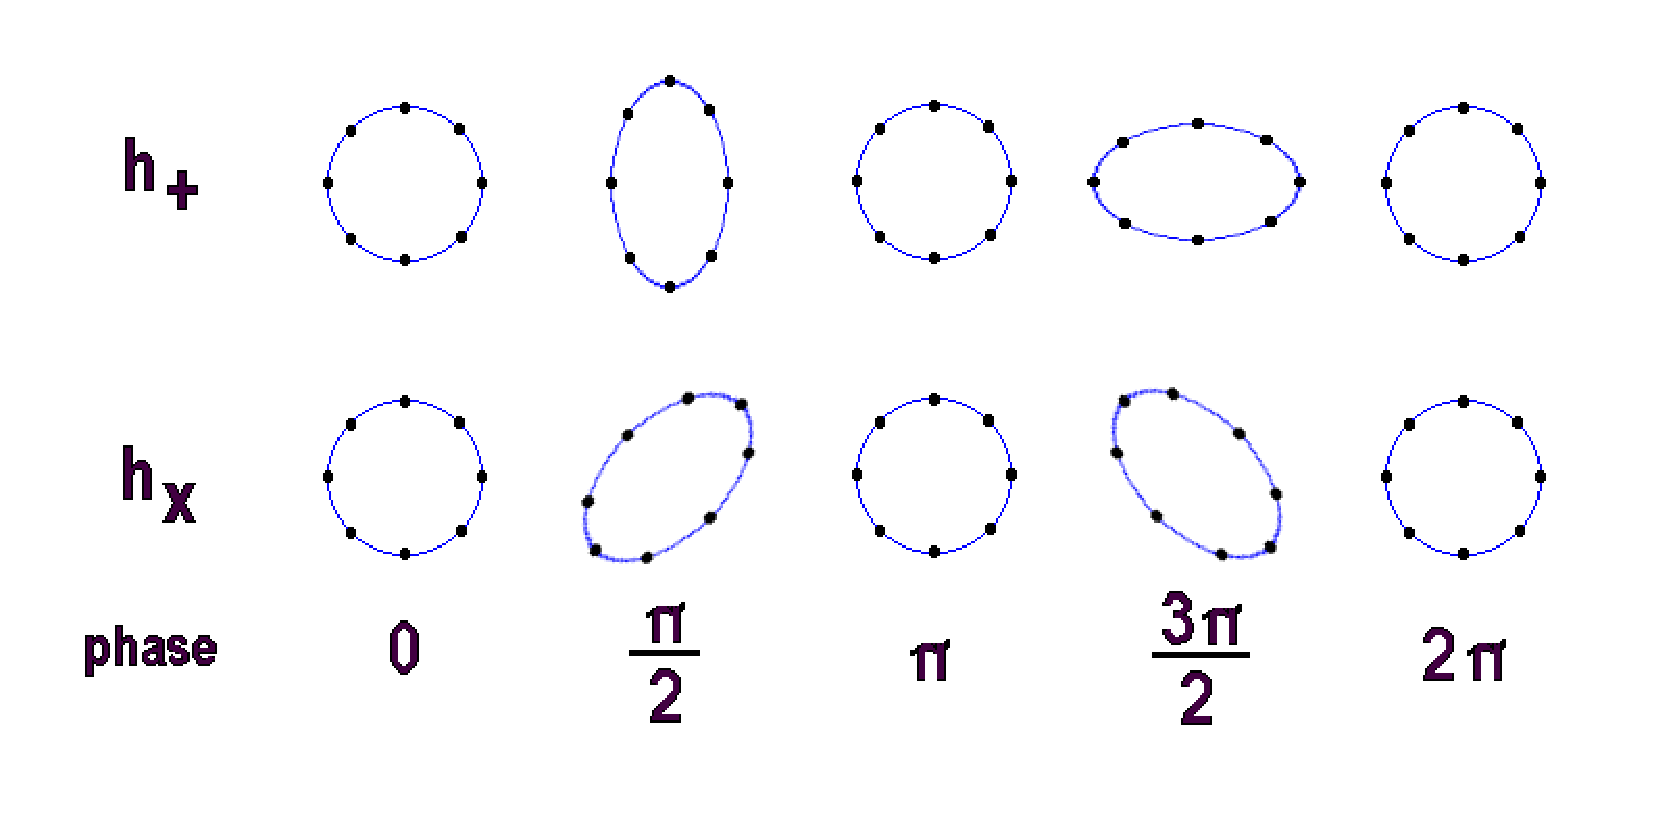
\includegraphics[width=150mm]{Images/rings.pdf}
    \caption{\label{fig:rings} The effect of a passing gravitational
      wave on a circle of test particles. The two different
      polarisations are at $45^\circ$ to each other. Figure reproduced
      with permission \cite{rings}.}
  \end{center}
\end{figure}

\subsection{The Experimental Setup}

We consider a one-dimensional system where the two neutrons with
opposite spins interact in a quantum harmonic oscillator. The two
particles are introduced in coherent states at rest on either side of
the potential. They will oscillate in the harmonic trap, interact and
eventually tunnel out. Repeating this experiment several times for the
same initial condition will reveal information about the state and
entanglement generated within the multilayer. If all unwanted effects
are reduced to acceptable levels then the results will depend on the
presence of gravitational waves if they have an effect on the
entanglement of the two neutrons.

Such a trap can be constructed using a multilayer of ultrathin
magnetic films of suitably chosen materials using molecular beam
epitaxy. The detailed behaviour of neutrons in such multilayers is
presented in \cite{blundell} where polarized neutron reflection was
used to study the magnetic properties of thin films. The potential
energy in the $\alpha$th region can be written as a sum of a nuclear
and magnetic term
\begin{equation}\label{eq:pot}
V_\alpha = \frac{\hbar^2}{2\pi m_n}\rho_\alpha b_\alpha -
\boldsymbol{\mu_n}\cdot\boldsymbol{B_\alpha},
\end{equation}
where $\boldsymbol{\mu_\alpha}$, $b_\alpha$, $\boldsymbol{B_\alpha}$
and $\rho_\alpha$ are the neutron moment, coherent nuclear scattering
length, magnetic field due to the magnetization in the region and
atomic density, respectively. The harmonic oscillator potential itself
can be formed from layers with no magnetization as long as the
thickness of a single film is much less than the particle wavelength
so the discrete nature of the material can be ignored. The second term
in \eqref{eq:pot} leads to different values for the potential
depending on the orientation of the neutron's spin relative to the
magnetic field. Hence, we can use magnetized layers as spin dependent
barriers. By placing such barriers at the two ends of the trap we
provide means for a spin measurement.

It has been shown that under certain approximations the quantum
dynamics of such a system are sufficient to generate maximally
entangled states under appropriate conditions \cite{edmund}. Producing
maximally entangled states with high fidelity is not necessary in this
experiment, but the work by Owen et al. provides a useful framework to
describe and model the entanglement in a harmonic trap.

The two particles are initialized separately such that their single
particle wave functions are spatially distinct at $t = 0$. We consider
neutrons, mass $m$, in a harmonic potential of the form $V =
\frac{1}{2}m \omega^2x^2$ initially in the coherent states
$\psi_{L/R}(x)$, where
\begin{equation}
\psi_R = A\exp\left( -\frac{m\omega}{2\hbar}(x - x_0)^2 \right) ,
\end{equation}
\begin{equation}
\psi_L(x) = \psi_R(-x),
\end{equation}
$x_0 > 0$ and $A$ is a normalization constant. To be spatially distinct, the
single particle wave functions must satisfy $\int_{-\infty}^0 \! \psi_R(x) \,
\mathrm{d} x \to 0$ and $\int^{\infty}_0 \! \psi_L(x) \, \mathrm{d} x
\to 0$. We can then write the initial two-particle state as
\begin{equation}
\begin{array} {lcl}
|\Psi(t=0)\rangle & = & \left( \int \!
\psi_L(x_1)a^\dagger_{\sigma_1}(x_1) \, \mathrm{d} x_1 \right) \left(
\int \! \psi_R(x_2)a^\dagger_{\sigma_2}(x_2) \, \mathrm{d} x_2 \right)
|0\rangle \\\\ & \equiv & \left( \int\int\Psi(x_1, x_2;
t=0)a^\dagger_{\sigma_1}(x_1)a^\dagger_{\sigma_2}(x_2) \mathrm{d} x_1
\mathrm{d} x_2 \right) |0\rangle \\\\ & \equiv &
|L_{\sigma_1}R_{\sigma_2}\rangle
\end{array}
\end{equation}
where $a^\dagger_{\sigma_i}(x_i)$ are the creation operators for a
neutron at $x_i$ with spin $\sigma_i$. We only consider neutrons which
are introduced into the trap with opposite spins, $\sigma_1 \neq
\sigma_2$, hence we can treat them as distinguishable. Therefore, the
creation operators commute.

The two-particle Hamiltonian for the two neutrons in the same harmonic
potential is given by
\begin{equation}\label{eq:hamiltonian}
\hat{H} = -\frac{\hbar^2}{2m}\left( \frac{\partial^2}{\partial x_1^2}
+ \frac{\partial^2}{\partial x_2^2} \right) +
\frac{1}{2}m\omega^2(x_1^2 + x_2^2) + V_{nn}(x_1-x_2)
\end{equation}
where $V_{nn}(x_1-x_2)$ is a translationally invariant potential between
the two neutrons and its exact form will be discussed in the next
section.

In the parity-dependent harmonic approximation, which assumes that the
spectrum of the Hamiltonian in \eqref{eq:hamiltonian} is equal to the
spectrum of a quantum harmonic oscillator except for a
parity-dependent energy shift, the wave function at integer
half-periods has been shown to be
\begin{equation}
|\Psi(t=n\pi/\omega)\rangle \propto
\cos\theta|L_{\sigma_1}R_{\sigma_2}\rangle +
e^{i\chi}\sin\theta|R_{\sigma_1}L_{\sigma_2}\rangle,
\end{equation}
where $\theta = n\pi\phi/2$, $\phi\hbar\omega$ is the energy shift
to the even parity eigenstates and $\chi$ is some phase \cite{edmund}.

